\documentclass{beamer}

\usepackage[italian]{babel}
\usepackage{graphicx}
\usepackage{url}
\usepackage{soul}
\usepackage{tikz}
\usepackage{listings}
\usepackage{xcolor}
\usepackage{algorithm}
\usepackage[noend]{algpseudocode}

\setbeamertemplate{navigation symbols}{}
\usetheme{default}
\usecolortheme{Nord}

% titolo, ...
\title{CoderFarm - Corso avanzato}
\subtitle{Lezione 0}
\author{Lorenzo Ferrari, Davide Bartoli}
\date{\today}

\begin{document}

\begin{frame}
    \titlepage
\end{frame}

\section{Introduzione}
\begin{frame}{Presentazione}{A chi è rivolto il corso?}
    Il corso avanzato \`e per chi sa gi\`a programmare e vuole avvicinarsi al mondo della Programmazione Competitiva (CP). \\
    Il nostro obiettivo \`e prepararvi per le Olimpiadi di Informatica (OIS/OII) e in generale per le gare di CP. \\
    \smallbreak
    Vi ricordiamo che:
    %
    \begin{itemize}
        \item In questo corso daremo per scontata una conoscenza di base della programmazione C++
        \item Le lezioni si svolgeranno con cadenza settimanale, il Mercoled\`i dalle 16.00
    \end{itemize}
    %
\end{frame}

\begin{frame}{Presentazione}{Quali argomenti tratteremo?}
    %
    \begin{block}{Tratteremo:}
        %
        \begin{itemize}
            \item Complessit\`a computazionale (a fini pratici)
            \item Ricorsione, Complete search e Backtracking.
            \item Programmazione dinamica
            \item Algoritmi sui Grafi
            \item Algoritmi greedy
            \item Strutture dati avanzate
            \item Algoritmi probabilistici
            \item Tecniche e ``trucchi'' anche inusuali
        \end{itemize}
        %
    \end{block}
    Il livello delle lezioni potr\`a essere aggiustato in base al vostro feedback.
    %
\end{frame}

\begin{frame}{Presentazione}{Chi siamo?}
    %
    \begin{itemize}
        \item \textbf{Nome:} Lorenzo Ferrari
        \item \textbf{Classe:} 2004
        \item \textbf{Provenienza:} Trento
        \item \textbf{Risultati alle OII:} due ori e un argento, primo posto OII 2022
        \item \textbf{Altri risultati olimpici:} menzione d'onore IOI, prima squadra italiana alle EOES
    \end{itemize}
    %
\end{frame}

\begin{frame}{Presentazione}{Chi siamo?}
    %
    \begin{itemize}
        \item \textbf{Nome:} Davide Bartoli
        \item \textbf{Classe:} 2003
        \item \textbf{Provenienza:} Imola
        \item \textbf{Risultati alle OII:} tre ori, primo posto OII 2020 e 2021
        \item \textbf{Altri risultati olimpici:} argento IOI, due ori alle olimpiadi di matematica
    \end{itemize}
    %
\end{frame}

\begin{frame}{Introduzione}{Gare di Informatica}
    %
    \begin{block}{Come funziona una gara di Informatica?}
        \begin{itemize}
            \item Dati i problemi, si scrivono dei programmi\footnote{quasi sempre in \textsc{C++}} che
                \begin{itemize}
                    \item prendono dei dati in \emph{input};
                    \item elaborano i dati per risolvere il problema;
                    \item ritornano i risultati in \emph{output}.
                \end{itemize}
            \item I programmi devono produrre la risposta corretta entro limiti di tempo e di memoria.
            \item Spesso i problemi hanno dei \emph{subtask} che forniscono \emph{punti parziali} 
            e guidano verso la soluzione del problema.
        \end{itemize}
    \end{block}
    %
\end{frame}

\begin{frame}{Introduzione}{Gare di Informatica}
    %
    Una soluzione deve essere:
    \pause
    \begin{itemize}
        \item \textbf{Corretta}: deve risolvere il problema
        \pause
        \item \textbf{Efficiente}: deve essere abbastanza veloce da trovare la soluzione entro il tempo limite
    \end{itemize}
    \pause
    Per controllare se una soluzione \`e efficiente possiamo stimare il numero di operazioni che il programma esegue calcolando la \textbf{complessit\`a computazionale} del programma, ovvero una stima del 
    numero di operazioni eseguite dal codice in funzione della dimensione dell'input.
    \pause 
    \vfill
    Calcolare la complessit\`a computazionale di un algoritmo permette di valutare se la soluzione \`e abbastanza veloce per risolvere il problema prima ancora di 
    scrivere il codice, facendo risparmiare tempo e fatica.
    %
\end{frame}

\section{Complessit\`a computazionale}
\begin{frame}{Complessit\`a Computazionale}{introduzione}
    La complessit\`a computazionale si esprime attraverso la notazione $O(f(N))$\footnote{letto ``O grande di $f(N)$''}, dove $f(N)$ \`e una funzione
    che stima il numero di operazioni eseguite dal programma in funzione della dimensione dell'input $N$.
    \pause
    \vfill
    Esempi:
    \begin{itemize}
        \item $O(1)$, l'algoritmo esegue sempre lo stesso numero di operazioni indipendentemente dall'input
        \pause
        \item $O(\log_2 N)$, esempio più tardi
        \pause
        \item $O(N)$, per esempio iterare sugli elementi di un array di dimensione $N$
        \pause
        \item $O(N^2)$, per esempio iterare sulle coppie di elementi
        \pause
        \item $O(2^N)$, per esempio iterare su tutti i sottoinsiemi
    \end{itemize}
\end{frame}

\begin{frame}{Complessit\`a Computazionale}{Caratteristiche}
    \begin{itemize}
        \item le operazioni elementari (+, *, -, /, $\dots$) sono considerate costanti: $O(1)$
        \pause
    \item dichiarazioni, assegnamenti, confronti di variabili semplici (\texttt{int}, \texttt{float}, $\dots$) sono considerati costanti: $O(1)$
        \pause
        \item input e output di variabili semplici sono considerati costanti: $O(1)$
        \pause
        \item ci interessano solo i termini pi\`u grandi: $O(N^2 + N + 1) = O(N^2)$
        \pause
        \item non ci interessano i fattori costanti: $O(10 \cdot N^2) = O(N^2)$
    \end{itemize}
\end{frame}

\begin{frame}{Esempio di calcolo della complessit\`a}{}
    \makebox[\textwidth]{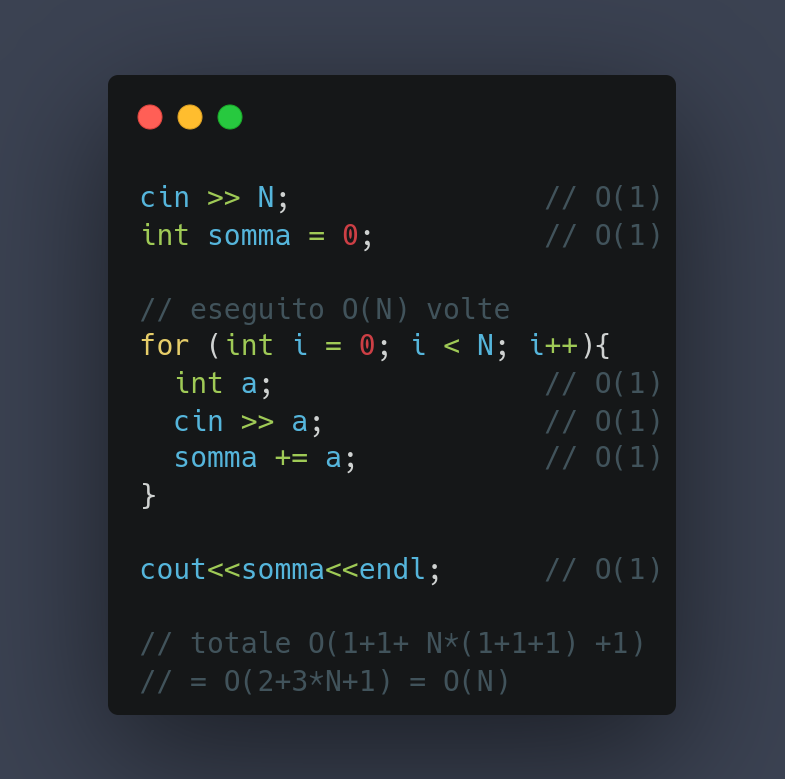
\includegraphics[scale=.30]{./img/O_N.png}}
\end{frame}

\begin{frame}{Esempio di calcolo della complessità}{}
    \makebox[\textwidth]{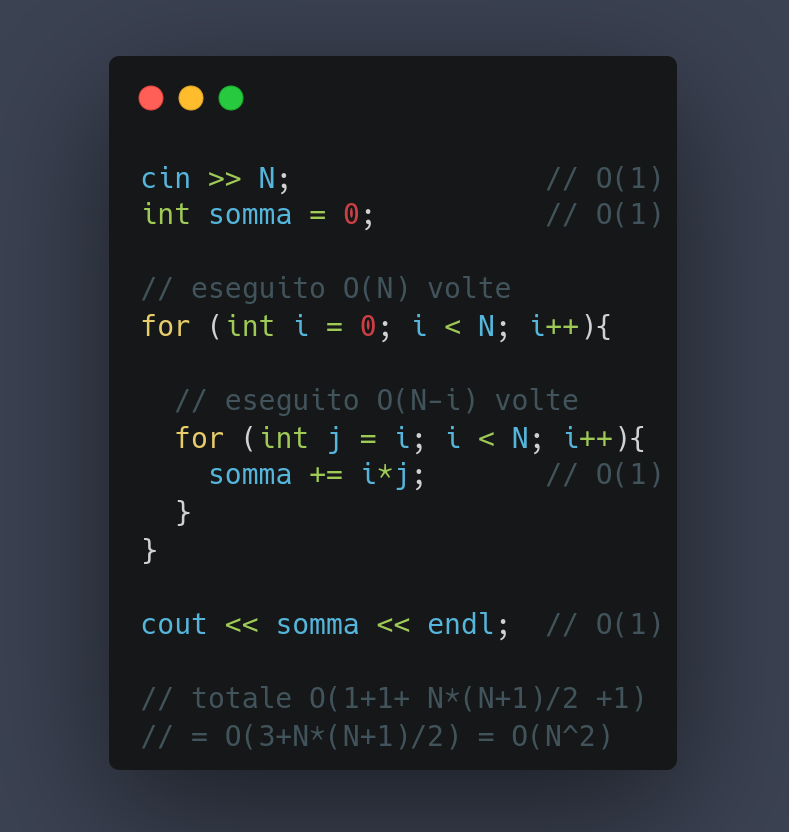
\includegraphics[scale=.30]{./img/O_N^2.png}}
\end{frame}

\begin{frame}[t]{Introduzione}{Problema di esempio}
    %
    \begin{exampleblock}{Lotteria di quadri}
    \textit{Data una sequenza di $N \leq 200 \ 000$ interi positivi e un intero $M$, trovare il massimo $B \leq N$ tale che la somma di ogni sottosegmento lungo $B$ sia al pi\`u $M$.}
    \end{exampleblock}
    \pause
    Come facciamo a controllare se un $B$ va bene?
    \pause
    \begin{itemize}
        \item per ogni $i = 0, 1, \dots, N-B$ possiamo controllare se la somma di $A[i], A[i+1], \dots, A[i+B-1]$ \`e al pi\`u $M$ in tempo $O(B)$.
        Dato che dobbiamo controllare ogni valore di $i$, il tempo totale \`e $O(NB)$. Questa soluzione \`e troppo lenta, cerchiamo di renderla pi\`u veloce.
    \end{itemize}
    %
\end{frame}

\begin{frame}{Controllo in $O(NB)$}{Implementazione}
    \makebox[\textwidth]{\includegraphics[scale=.30]{./img/works\_slow.png}}
\end{frame}

\begin{frame}[t]{Introduzione}{Problema di esempio}
    Possiamo fare meglio?
    \pause
    \begin{itemize}
        \item possiamo notare che stiamo calcolando pi\`u volte le stesse somme. In particolare conoscendo la somma di $A[i], A[i+1], \dots, A[i+B-1]$ possiamo
        facilmente calcolare la somma di $A[i+1], A[i+2], \dots, A[i+B]$ senza dover ricalcolare tutto da capo. 
        \pause
        \item chiamiamo $K$ la somma di $A[i], A[i+1], \dots, A[i+B-1]$. Allora possiamo calcolare la somma di $A[i+1], A[i+2], \dots, A[i+B]$ in tempo $O(1)$ come $K - A[i] + A[i+B]$.
        \pause
        \item in questo modo possiamo controllare se un $B$ va bene in tempo $O(B+(N-B))=O(N)$.
    \end{itemize}
    %
\end{frame}

\begin{frame}{Controllo in $O(N)$}{Implementazione}
    \makebox[\textwidth]{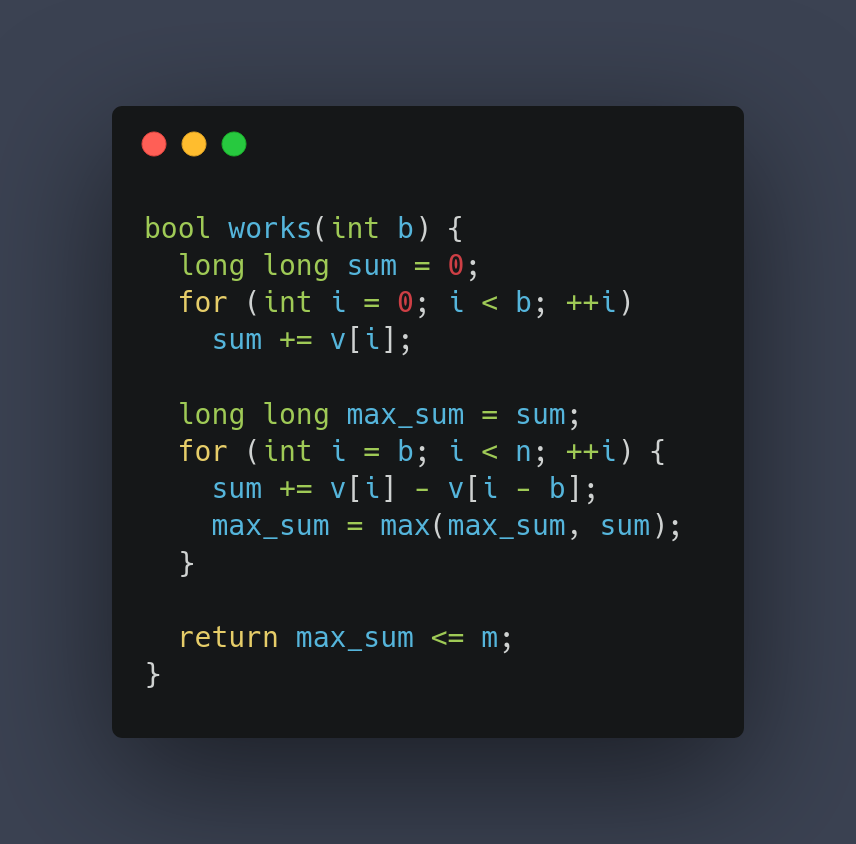
\includegraphics[scale=.30]{./img/controllo.png}}
\end{frame}

\begin{frame}[t]{Introduzione}{Problema di esempio}
    \begin{itemize}
        \item ora sappiamo controllare se un $B$ va bene in tempo $O(N)$. Come possiamo trovare il massimo $B$ che va bene?
        \pause
        \item possiamo controllare $B = j$ per $j = 0, 1, \dots, N$ e prendere il pi\`u grande valore valido. Questo ha complessit\`a $O(N^2)$
        \pause
        \item ahim\`e $(2 \cdot 10^5)^2$ operazioni sono decisamente troppe per 2 secondi
        \pause
        \item si pu\`o fare meglio di cos\`i?
    \end{itemize}
    %
\end{frame}

\begin{frame}[t]{Introduzione}{Problema di esempio}
    %
    \begin{exampleblock}{Lotteria di quadri}
    \textit{Data una sequenza di $N \leq 200 \ 000$ interi positivi e un intero $M$, trovare il massimo $B \leq N$ tale che la somma di ogni sottosegmento lungo $B$ sia al pi\`u $M$.}
    \end{exampleblock}
    %
    Osservazioni:
    \begin{itemize}
        \item se $B_x$ \`e valido, allora $B_y < B_x$ \`e anch'esso valido
        \item se $B_x$ \`e non valido, allora $B_y > B_x$ \`e anch'esso non valido
    \end{itemize}
    %
    \pause
    %
    Con queste premesse esiste un algoritmo che ci permette di trovare il pi\`u grande $B_x$ valido con pochi confronti!
\end{frame}

\begin{frame}{Ricerca binaria}{Algoritmo}
    %
    \begin{exampleblock}{Definizione del problema}
        Dato un array potenzialmente molto grande della forma $[\dots, 0, 0, 0, 1, 1, 1, \dots]$, trova l'ultimo $0$.
    \end{exampleblock}
    %
    \pause
    Una possibile soluzione \`e controllare tutti gli elementi dell'array in ordine e fermarci 
    quando troviamo un $1$. Qusta soluzione è corretta ma non è efficiente, infatti ha complessità $O(N)$.
    Possiamo fare meglio, sfruttando il fatto che tutti gli $0$ sono prima di tutti gli $1$?
    %
    \vfill
    \small{\underline{\url{https://forum.olinfo.it/t/7224}}}
\end{frame}

\begin{frame}{Ricerca binaria}{Algoritmo}
    \begin{block}{Idea}
        Per cercare una determinata pagina in un libro nessuno scorre pagina per pagina dall'inizio.
        \`E molto pi\`u pratico aprire circa a met\`a, controllare in che met\`a si trova la pagina che cerchiamo, e cos\`i finch\'e non abbiamo finito.
    \end{block}
    \pause
    %
    Algoritmo:
    \begin{itemize}
        \item iniziamo con un intervallo $[l, r)$
        \pause
        \item controlliamo $mid = (l + r) / 2$
        \item se $mid$ è $0$, allora la risposta si trova in $[mid, r)$
        \item altrimenti la risposta si trova in $[l, mid)$
    \end{itemize}
    \pause
    Ripetiamo questo processo finchè l'intervallo $[l, r)$ non ha dimensione $1$
    (ovvero $l = r - 1$). L'unico elemento rimasto è la risposta che stavamo cercando.
\end{frame}

\begin{frame}{Ricerca binaria}{Complessit\`a di tempo}
    %
    \begin{itemize}
        \item Lo spazio di ricerca \`e inizialmente $N$, poi viene dimezzato ad ogni iterazione finch\'e non rimane un solo elemento.
        \pause
        \item Quindi inizialmente abbiamo $N$ possibili candidati, poi $N/2$, poi $N/4$, e cos\`i via.
        \pause
        \item In totale sono sufficienti $\lceil \log_2 N \rceil$ iterazioni e controlli.
        \begin{exampleblock}{Logaritmo}
        Il logaritmo in base 2 di $N$ \`e il numero di volte che bisogna moltiplicare $2$ per ottenere $N$.
        $$\log_2 N = x \iff 2^x = N$$
        Questo valore cresce molto lentamente, per esempio $\log_2 10^6 \approx 20$.
        \end{exampleblock}
    \end{itemize}
    \pause
    \break
    A differenza della ricerca lineare, la ricerca binaria \`e applicabile anche su spazi di ricerca molto grandi.
\end{frame}

\begin{frame}{Ricerca binaria}{Implementazione}
    \makebox[\textwidth]{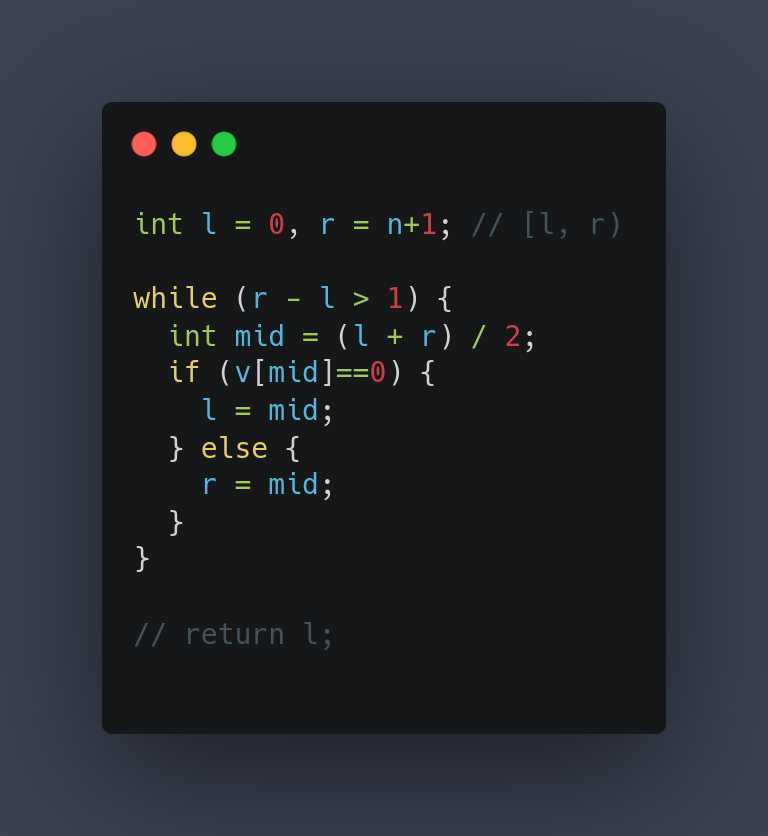
\includegraphics[scale=.30]{./img/binarysearch1.png}}
\end{frame}
%
\begin{frame}[t]{Introduzione}{Problema di esempio}
    Ritorniamo ora al problema precedente.
    Avevamo osservato che:
    \begin{itemize}
        \item se $B_x$ \`e valido, allora $B_y < B_x$ \`e anch'esso valido
        \item se $B_x$ \`e non valido, allora $B_y > B_x$ \`e anch'esso non valido
    \end{itemize}
    \pause
    Possiamo quindi immaginare un array in cui ogni elemento \`e $0$ se $B_x$ \`e valido, $1$ altrimenti.\\
    \pause
    Questo array è della forma $[\dots, 0, 0, 1, 1, \dots]$.
    \pause
    Possiamo quindi utilizzare la ricerca binaria per trovare la risposta velocemente!
    \pause
    \begin{itemize}
        \item sappiamo controllare se un certo $B$ \`e valido in $O(N)$
        \pause
        \item possiamo usare la ricerca binaria per trovare il pi\`u grande $B$ valido facendo $O(\log N)$ controlli.
    \end{itemize}
    La complessità totale \`e quindi $O(N \log N)$, che \`e sufficiente per entrare nel limite di tempo.    
\end{frame}

\begin{frame}{Qui potete testare le vostre soluzioni}
    %
    \small{\underline{\url{https://training.olinfo.it/\#/task/abc_quadri/statement}}}
    %
    \begin{exampleblock}{Lotteria di quadri}
    \textit{Data una sequenza di $N \leq 200 \ 000$ interi positivi e un intero $M$, trovare il massimo $B \leq N$ tale che la somma di ogni sottosegmento lungo $B$ sia al pi\`u $M$.}
    \end{exampleblock}
\end{frame}

\begin{frame}{Problemi addizionali}
    \underline{\url{https://training.olinfo.it/\#/task/ois_tickets/statement}}
    \underline{\url{https://training.olinfo.it/\#/task/ois_annoluce/statement}}
\end{frame}

\end{document}
